\chapter{\textsf{\acronym}}
\section*{Descrição}
O NUXIS é uma ferramenta de gestão centralizada de recursos disponíveis numa rede. Consiste numa distribuição linux pré-instalada e configurada, que permite fazer a gestão via rede de servidores e seus recursos.

O NUXIS encontra-se dividida principalmente em dois blocos funcionais:

\begin{itemize}
	\item \emph{Central Management} (CM)
        \item \emph{Virtualization Agent} (VA)
\end{itemize}

\begin{figure}[H]
	\begin{center}
	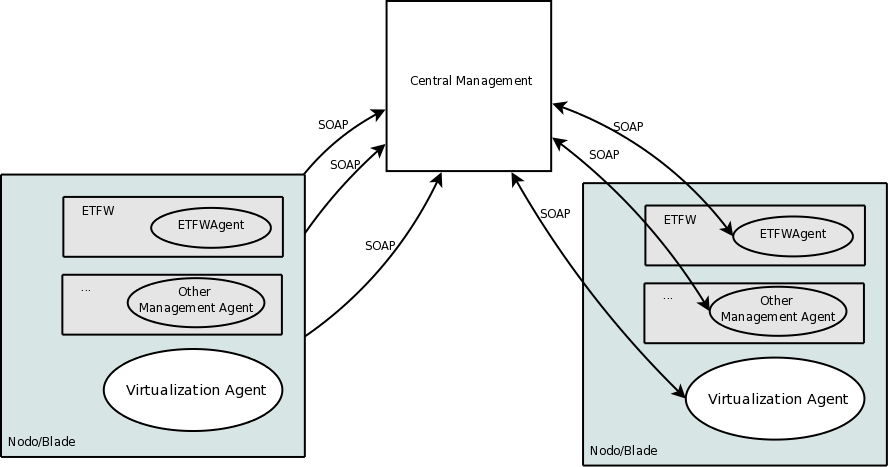
\includegraphics[scale=0.35]{screenshots/etva_blocos.png}
	\caption{Esquema geral do NUXIS}
	\label{fig:etva_blocos}
	\end{center}
\end{figure}

O CM é o bloco responsável por gerir toda a infra-estrutura.
Os \emph{Virtualization Agents} são responsáveis pelo processamento dos pedidos entre os servidores de virtualização (\emph{nodes}) e o CM.

Dentro de um servidor de virtualização(\emph{node}) poderão existir máquinas virtuais com \emph{Management Agents}. Estes agentes, permitem a gestão ao nível dos serviços/aplicações instalados na máquina virtual (ver figura \ref{fig:etva_blocos} ).

No \acronym, existem vários servidores de virtualização (\emph{nodes}) a comunicar com o CM. A configuração da rede inicial, é efectuada, com recurso a VLANs, através do \emph{Assistente de configuração inicial} conforme indica a figura \ref{fig:first_time_wizard}.
\begin{figure}[H]
    \begin{center}
	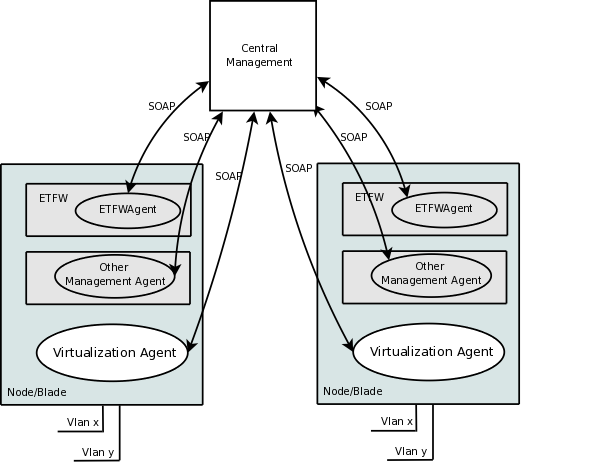
\includegraphics[scale=0.6]{screenshots/etva_enterprise.png}
	\caption{Modelo \acronym}
	\label{fig:etva_enterprise}
	\end{center}
\end{figure}
 
Este manual de utilização/configuração descreve a ferramenta de gestão, o CM (\emph{Central Management}).

\pagebreak
\chapter{\textsf{Instalação}}
\label{chp:installation}
\section{Versão enterprise}

Para efectuar a instalação deveremos utilizar o CD-ROM com a imagem da instalação do NUXIS e proceder ao arranque pelo mesmo.

Na versão \emph{enterprise}, deveremos ter disponível uma máquina para instalação da interface de gestão (\emph{Central Management}) e proceder à instalação de cada uma das máquinas dos servidores de virtualização.

\begin{figure}[H]
	\begin{center}
	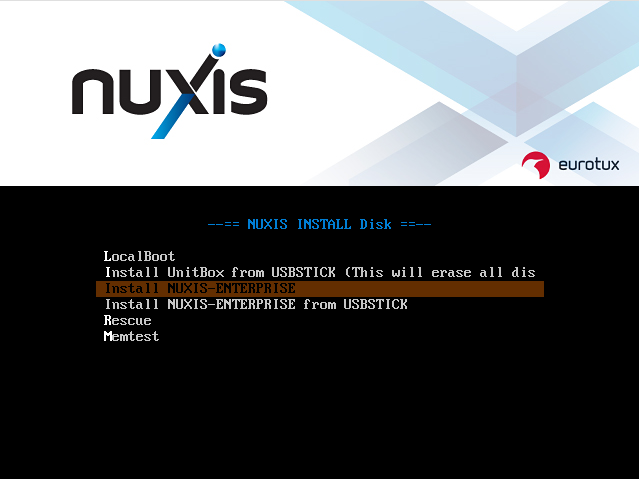
\includegraphics[scale=0.4]{screenshots/install/nuxis/bootmenu.png}
	\caption{Menu de instalação da versão Enterprise}
	\label{fig:boot_install_screen_enterprise}
	\end{center}
\end{figure}

Em ambos os casos, após o arranque por CD-ROM, devemos escolher a opção \emph{Install NUXIS-ENTERPRISE} e seguir aos passos de instalação.

\begin{figure}[H]
	\begin{center}
	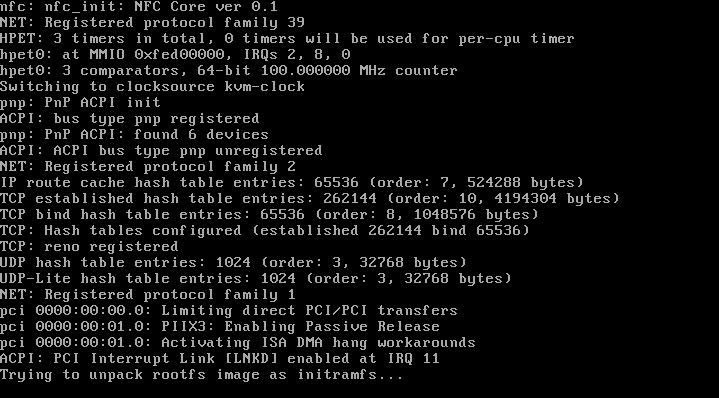
\includegraphics[scale=0.3]{screenshots/install/nuxis/boot_installer.png}
	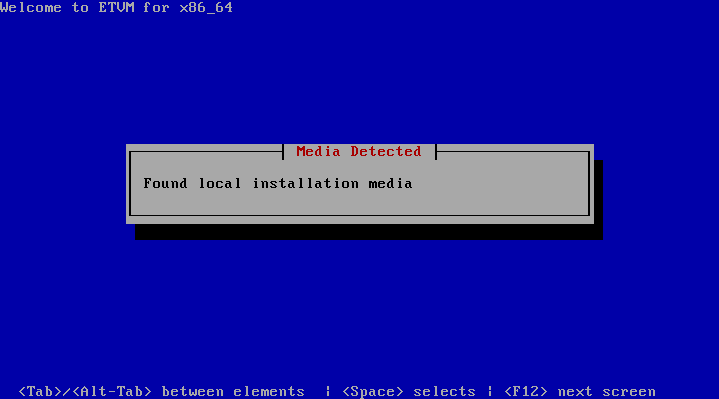
\includegraphics[scale=0.3]{screenshots/install/nuxis/load_installer_01.png}
	%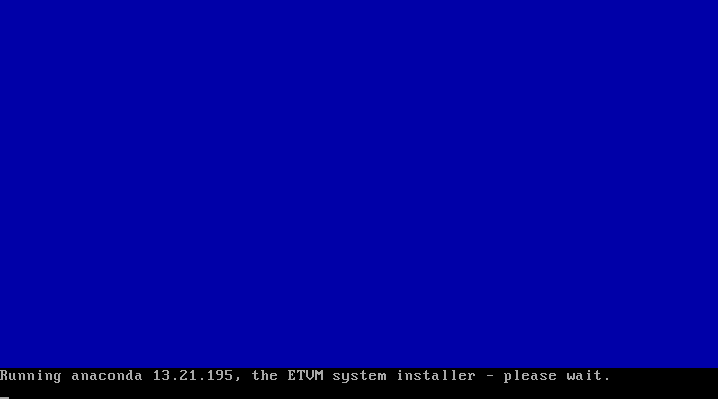
\includegraphics[scale=0.4]{screenshots/install/nuxis/load_installer_02.png}
	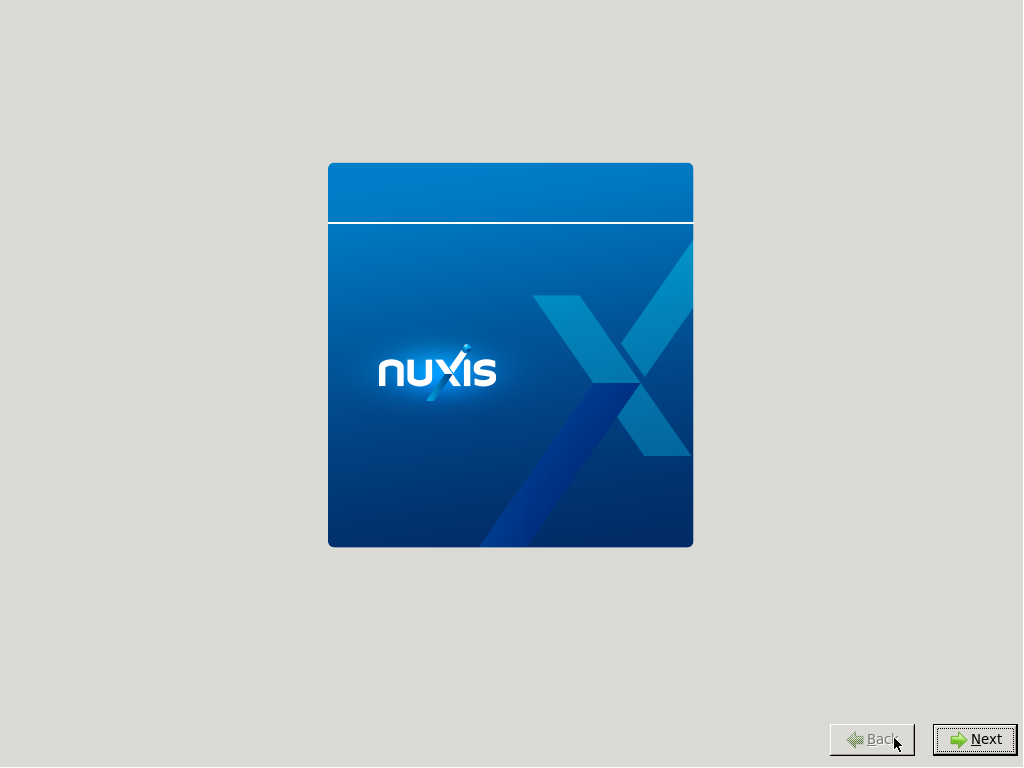
\includegraphics[scale=0.3]{screenshots/install/nuxis/wizard_install_01.png}
    \caption{Instalação da versão Enterprise - Arranque}
	\label{fig:installation_enterprise_01}
	\end{center}
\end{figure}
\begin{figure}[H]
	\begin{center}
	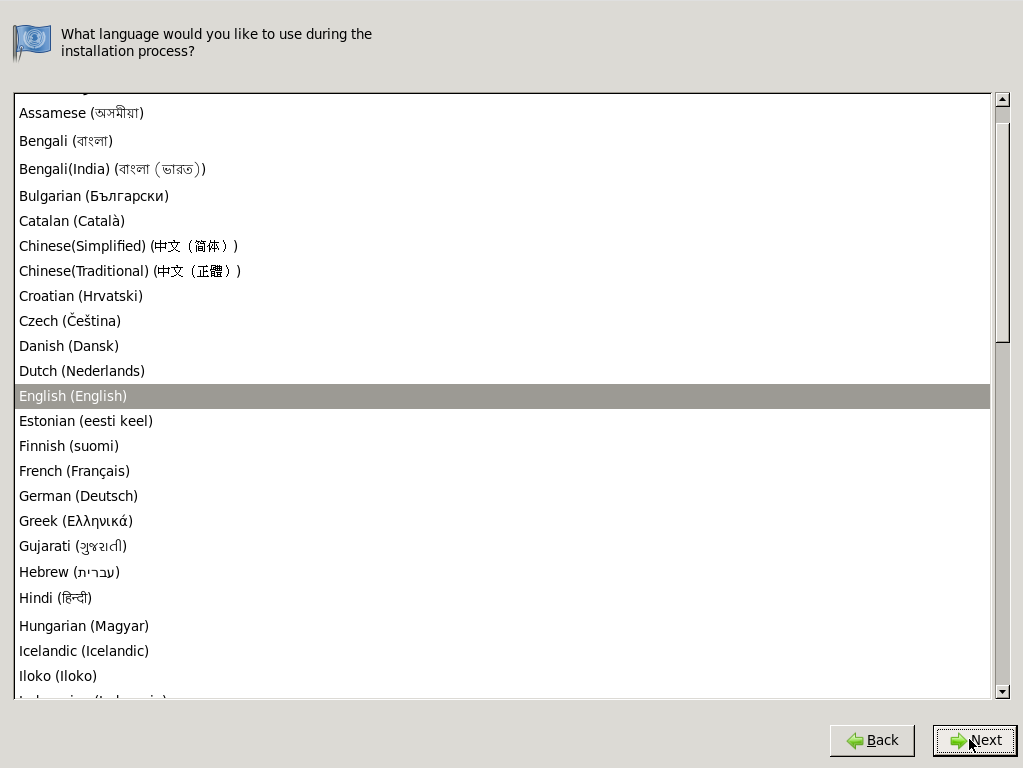
\includegraphics[scale=0.2]{screenshots/install/nuxis/wizard_install_02.png}
	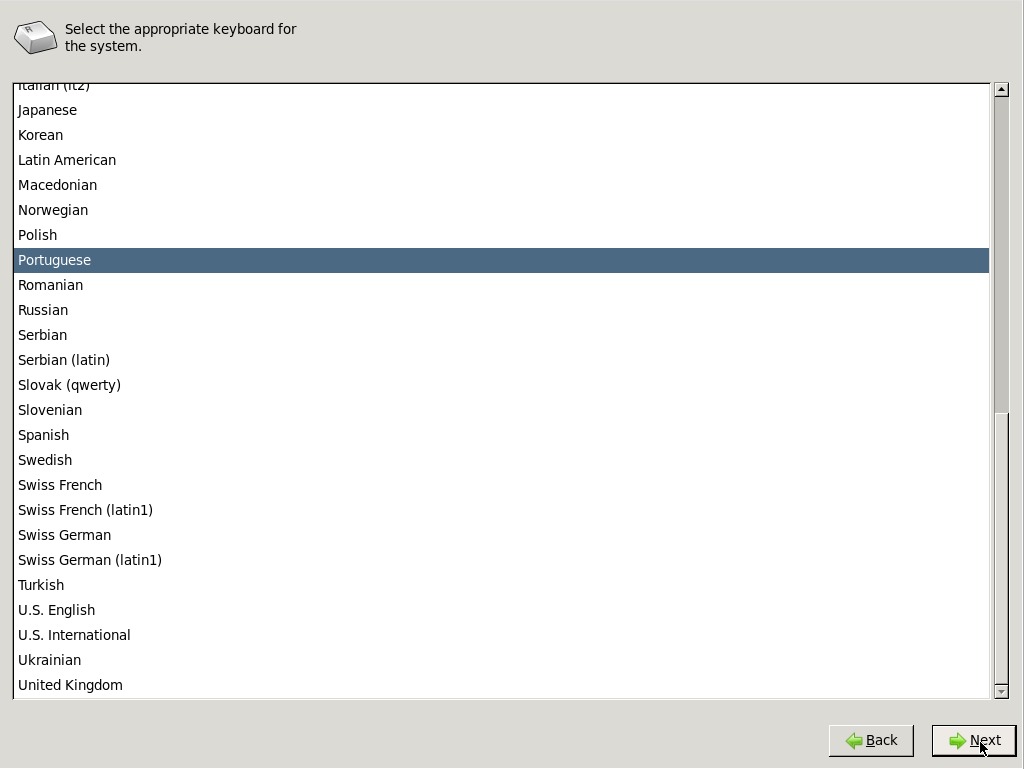
\includegraphics[scale=0.2]{screenshots/install/nuxis/wizard_install_03.png}
	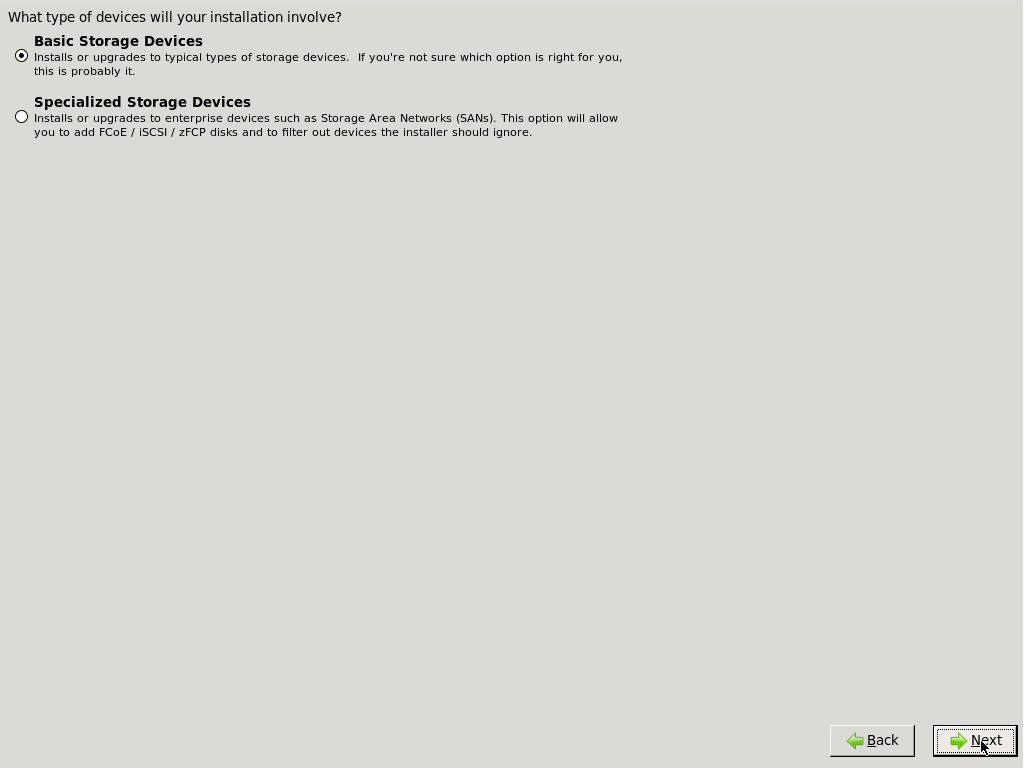
\includegraphics[scale=0.2]{screenshots/install/nuxis/wizard_install_04.png}
	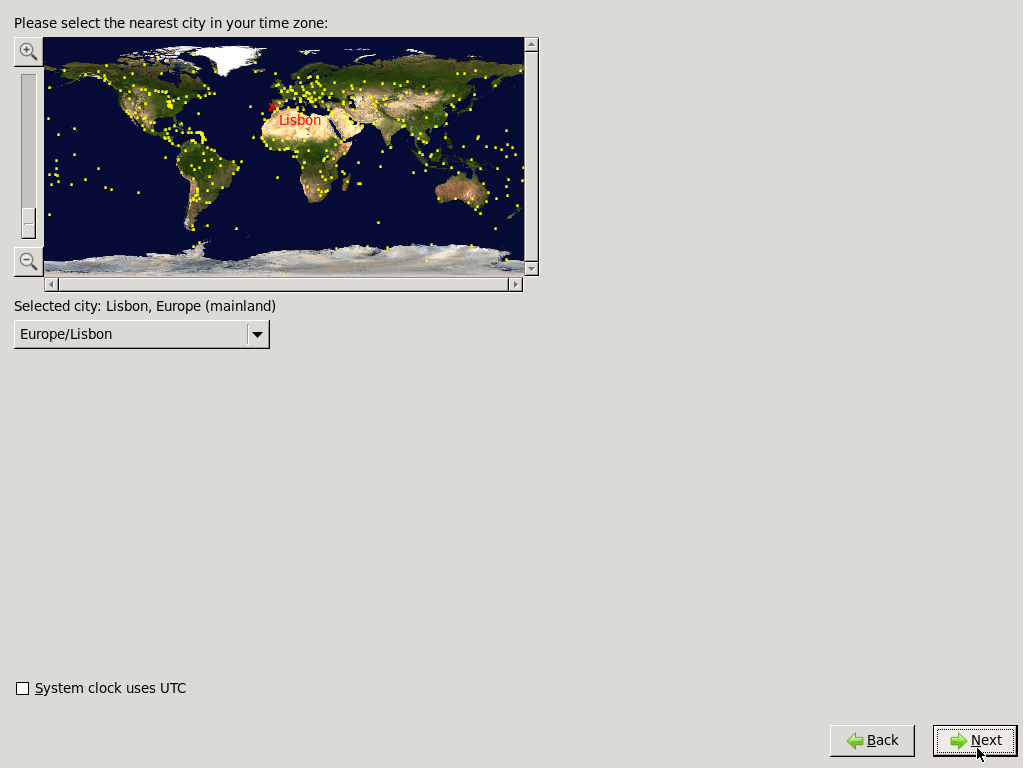
\includegraphics[scale=0.2]{screenshots/install/nuxis/wizard_install_05.png}
	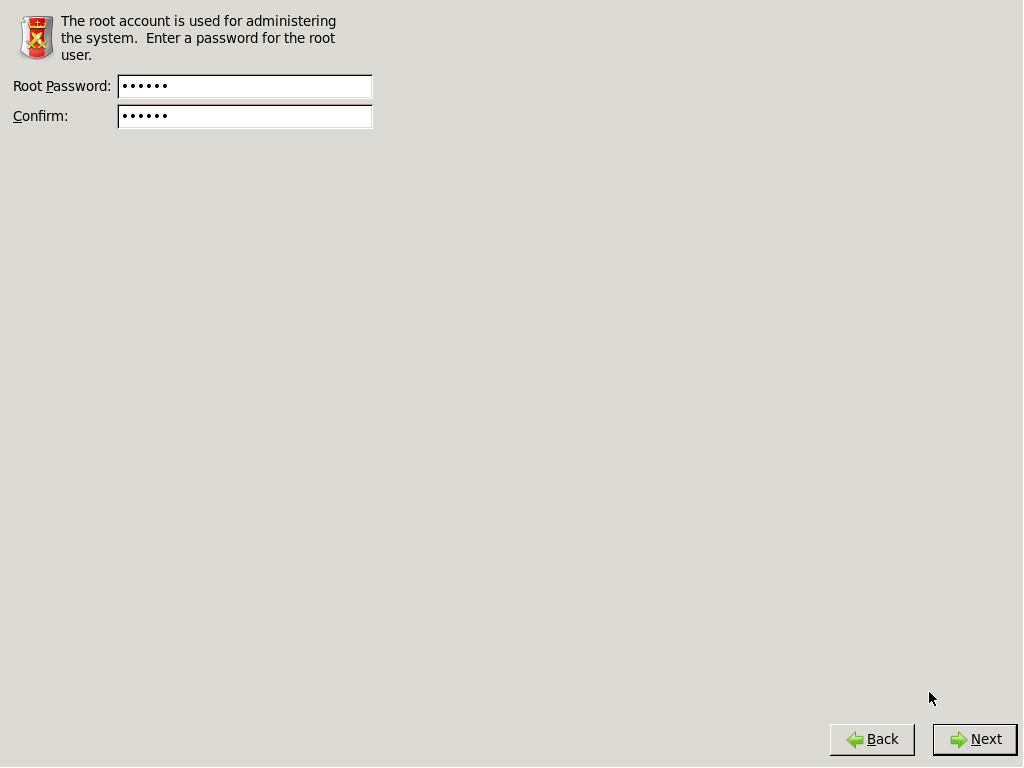
\includegraphics[scale=0.2]{screenshots/install/nuxis/wizard_install_06.png}
	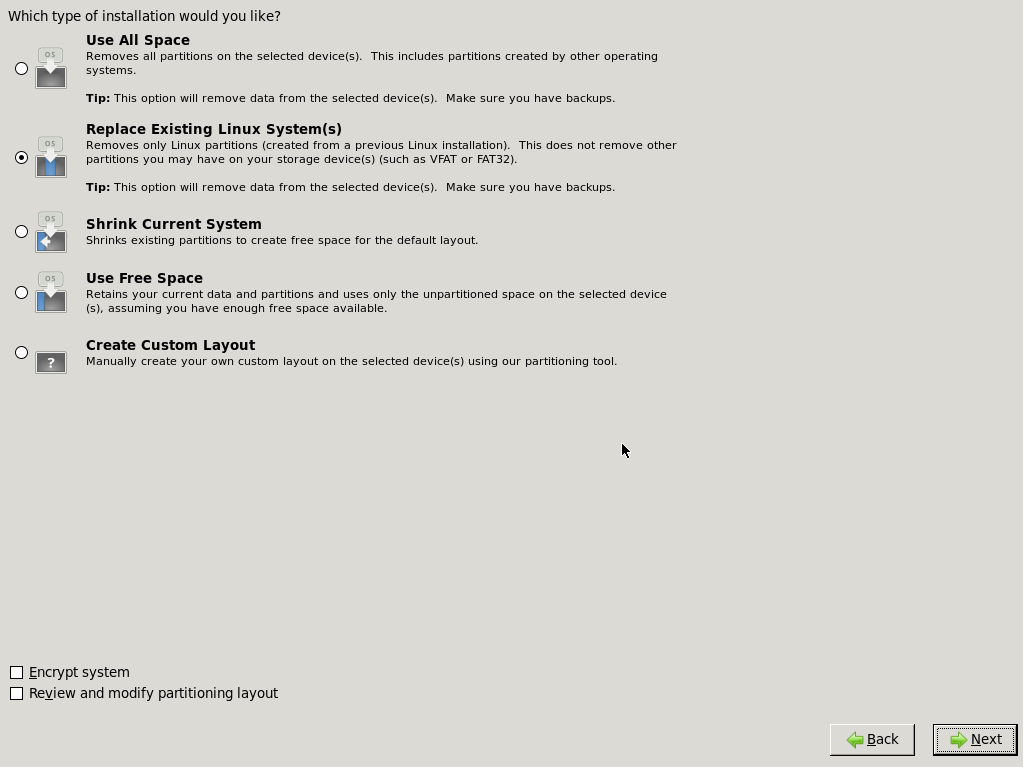
\includegraphics[scale=0.2]{screenshots/install/nuxis/wizard_install_07.png}
    \caption{Instalação da versão Enterprise - Configuração da instalação}
	\label{fig:installation_enterprise_02}
	\end{center}
\end{figure}
\begin{figure}[H]
	\begin{center}
	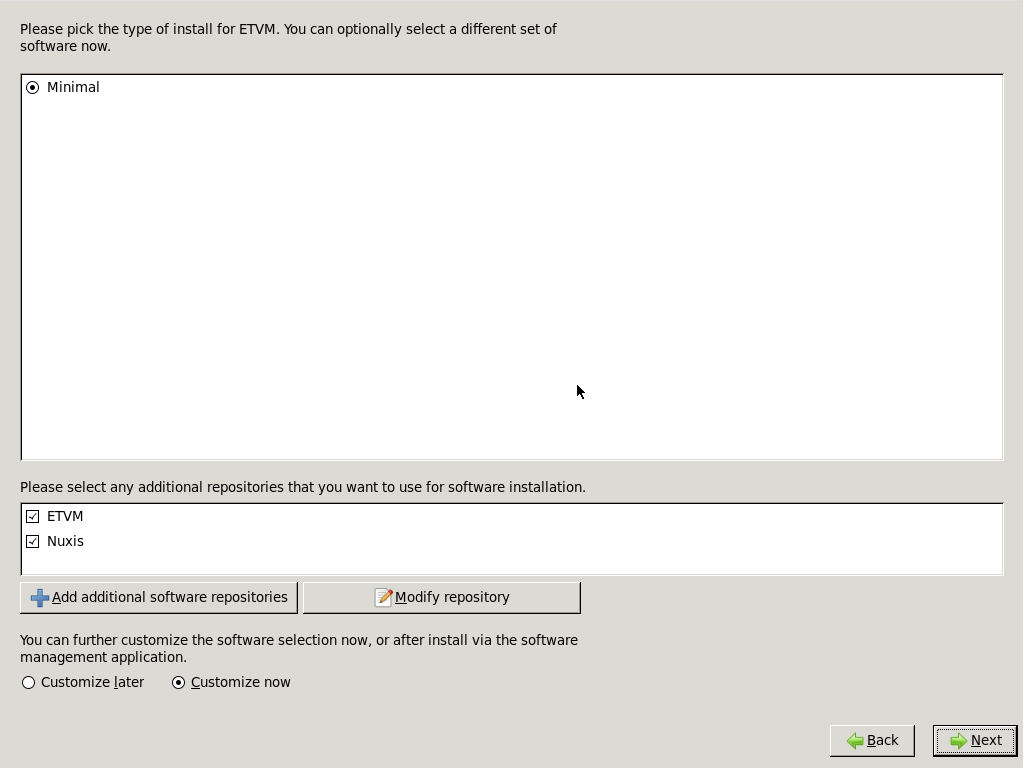
\includegraphics[scale=0.2]{screenshots/install/nuxis/packages_selection_01.png}
	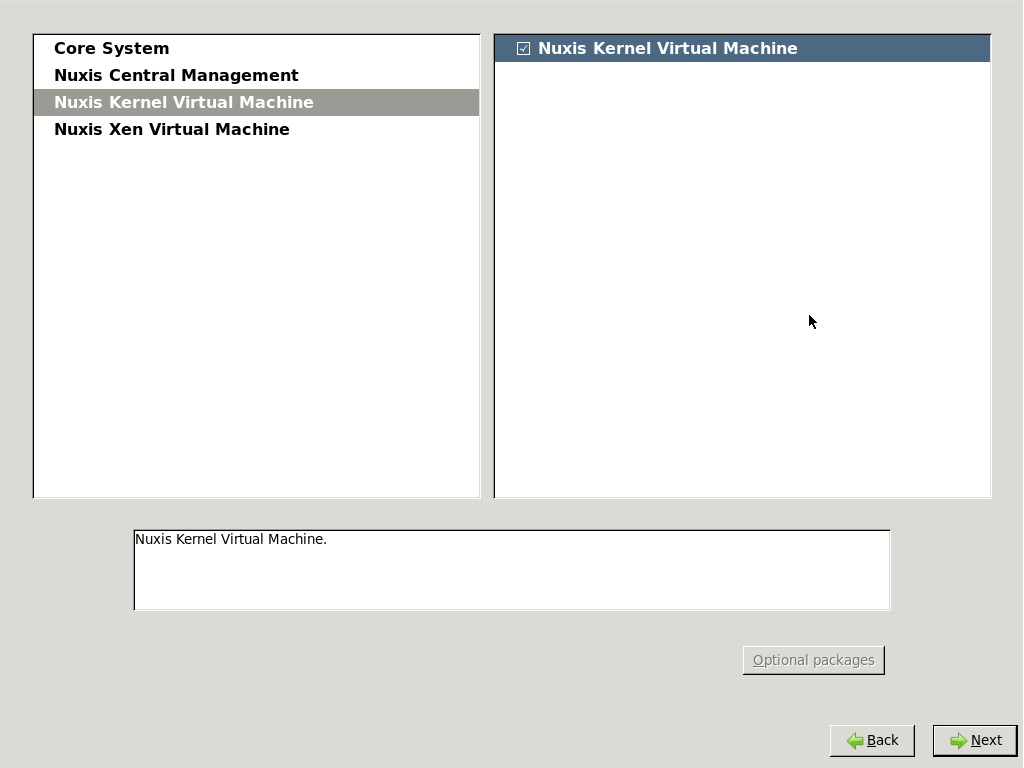
\includegraphics[scale=0.2]{screenshots/install/nuxis/packages_selection_02.png}
    \caption{Instalação da versão Enterprise - Pacotes}
	\label{fig:installation_enterprise_05}
	\end{center}
\end{figure}
Na escolha dos pacotes para instalação deveremos escolher \emph{Nuxis Central Management} para instalar a interface de gestão, \emph{Nuxis Kernel Virtual Machine} para instalar o servidor de virtualização com suporte para KVM ou \emph{Nuxis Xen Virtual Machine} para instalar o sevidor de virtualização com suporte para XEN.

\begin{figure}[H]
	\begin{center}
	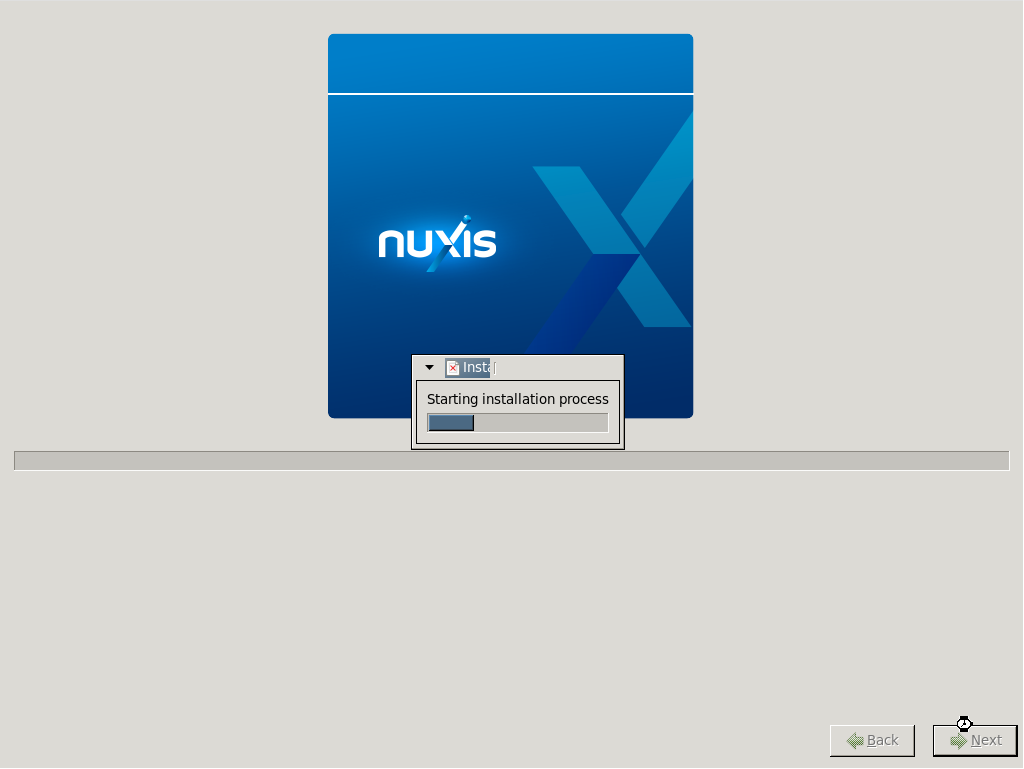
\includegraphics[scale=0.2]{screenshots/install/nuxis/start_install.png}
	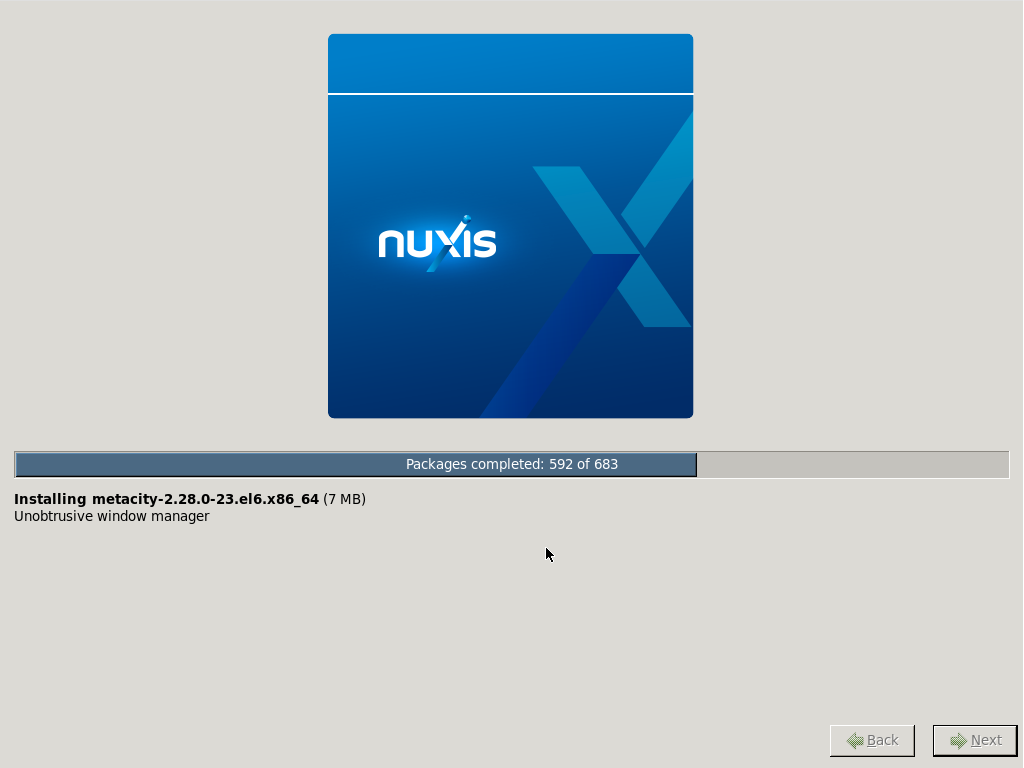
\includegraphics[scale=0.2]{screenshots/install/nuxis/install_progress_02.png}
	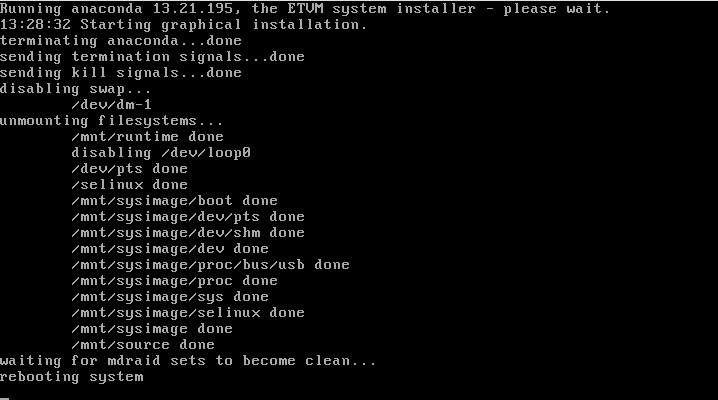
\includegraphics[scale=0.4]{screenshots/install/nuxis/install_reboot.png}
    \caption{Instalação da versão Enterprise - Conclusão}
	\label{fig:installation_enterprise_06}
	\end{center}
\end{figure}

Após a instalação, procedemos ao arranque do servidor e respectiva configuração de rede.

\begin{figure}[H]
	\begin{center}
    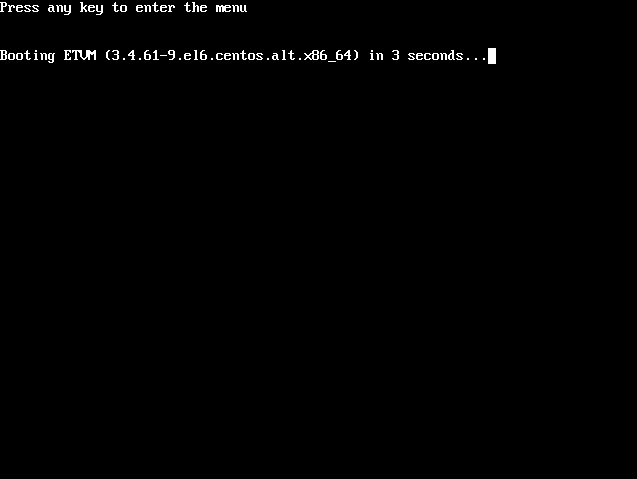
\includegraphics[scale=0.4]{screenshots/install/nuxis/pos_install_bootmenu.png}
    \caption{Configuração após a instalação - Arranque}
	\label{fig:installation_enterprise_pos_01}
	\end{center}
\end{figure}

\begin{figure}[H]
	\begin{center}
    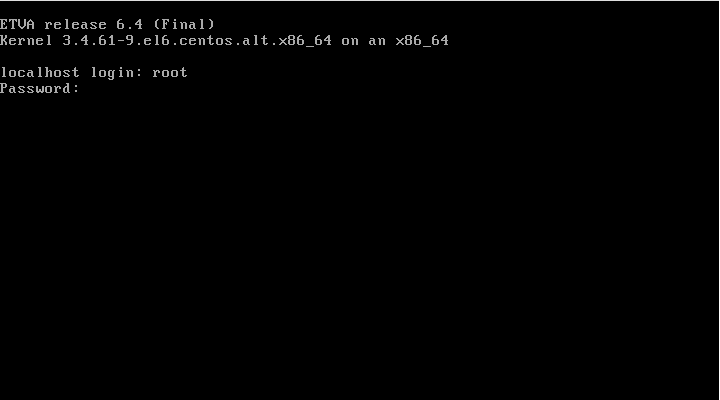
\includegraphics[scale=0.3]{screenshots/install/nuxis/login.png}
    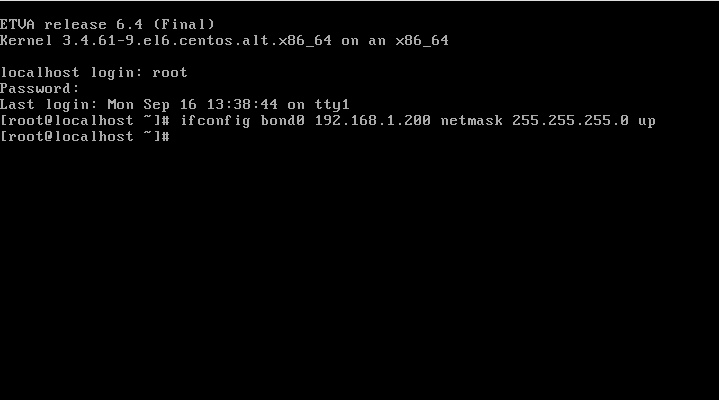
\includegraphics[scale=0.3]{screenshots/install/nuxis/configure_network.png}
    \caption{Configuração após a instalação - Login e configuração de rede}
	\label{fig:installation_enterprise_pos_02}
	\end{center}
\end{figure}

Para configurar a rede, acedemos à consola da máquina com \emph{login} \emph{root} e respectiva \emph{password} e atribuímos um endereço IP.

\begin{figure}[H]
	\begin{center}
    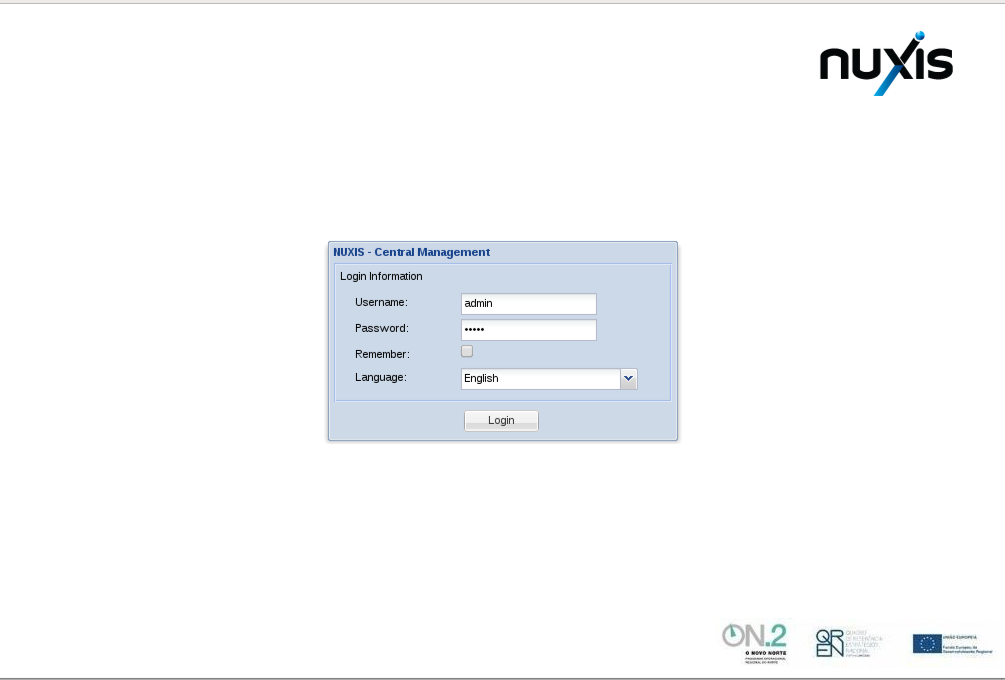
\includegraphics[scale=0.4]{screenshots/install/nuxis/nuxis_enterprise_pos_install_21.png}
    \caption{Configuração após a instalação - Autenticação}
	\label{fig:installation_enterprise_pos_03}
	\end{center}
\end{figure}

A seguir acedemos à interface de gestão apartir do endereço configurado anteriormente e autenticamos como o utilizador \emph{admin} e a \emph{password} \emph{default} (\emph{admin}).

\begin{figure}[H]
	\begin{center}
    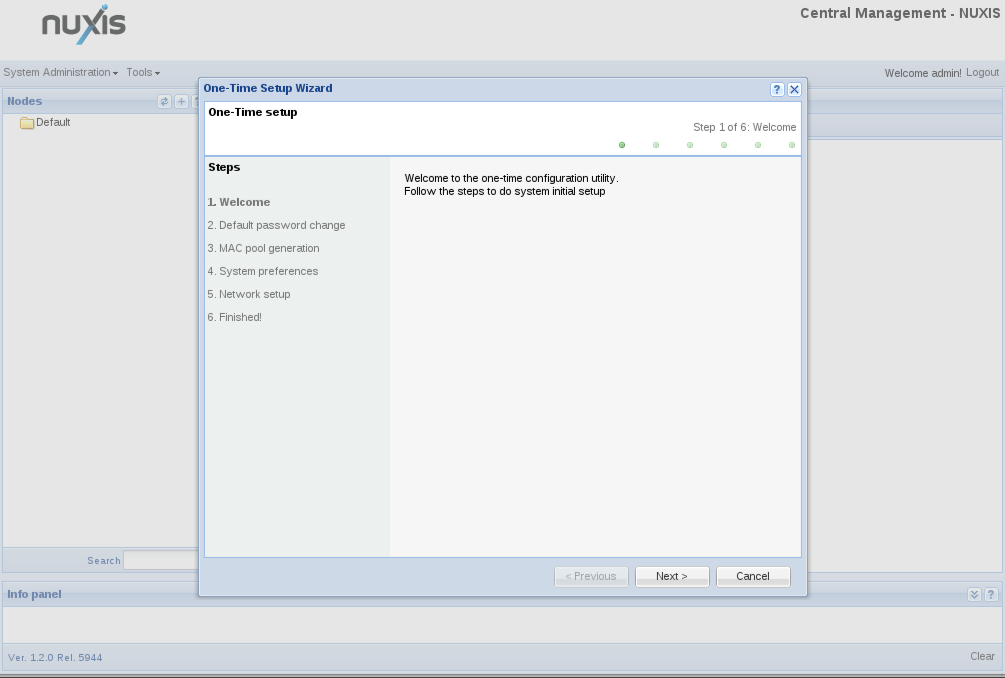
\includegraphics[scale=0.4]{screenshots/install/nuxis/nuxis_enterprise_wiz_install_22.png}
    \caption{Configuração após a instalação - Configuração inicial}
	\label{fig:installation_enterprise_wiz_01}
	\end{center}
\end{figure}

No primeiro acesso, somos solicitados a efectuar a configuração inicial para alteração de password, geração da MAC pool, preferências de conectividade e configuração de rede, tal como referido em  \ref{fig:first_time_wizard}.

\begin{figure}[H]
	\begin{center}
    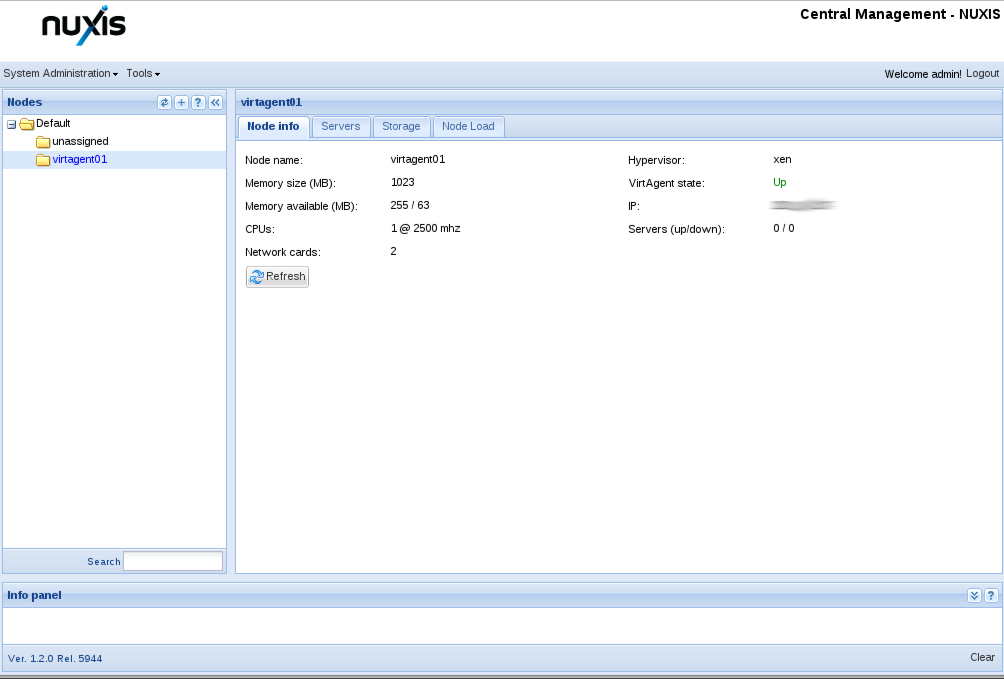
\includegraphics[scale=0.4]{screenshots/install/nuxis/nuxis_enterprise_wiz_install_28.png}
    \caption{Configuração após a instalação - Servidor de virtualização}
	\label{fig:installation_enterprise_wiz_02}
	\end{center}
\end{figure}

Depois de proceder à configuração da máquina de gestão e de instalar o servidor de virtualização, este deverá aparecer registado na interface e pronto para ser autorizado para ser passível de ser gerido por esta interface.

\pagebreak
